% Chapter 5 -- Results
% Status: sections 5.1, 5.3, 5.4 and 5.7 have audited numbers; 5.2 partial; 5.5 partial;
% 5.6 pending (privacy measurements). Every number is a macro or an \input table.
\chapter{Results}
\label{ch:results}

\section{Main Comparison of the Four Placements}
\label{sec:res-main}

Table~\ref{tab:main} reports the full-population metrics of the four methods at their best
round, and Figure~\ref{fig:group-bars} the \ndcg{} by user group. Three observations carry
through the rest of the chapter.

\begin{table}[htbp]
  \caption{Main comparison on MovieLens 1M, $N=\NClients$, $C=\ParticipationC$, $R=\NRounds$,
  full-population scoring at the restored best round. $^{\ddagger}$Centralised BPR-MF with the
  same leave-one-out and 99-negative protocol but an untuned configuration ($d=\CentralBprDim$,
  \CentralBprEpochs{} epochs, \CentralBprNeg{} negative); the PFedRec paper reports
  \PublishedCentralMfNdcg{} for a tuned centralised MF, so ``federated beats centralised'' is not
  claimed.}
  \label{tab:main}
  \centering\small
  % AUTO-GENERATED by thesis/scripts/build_assets.py -- do not edit by hand.
% final_metrics.best of each run (6040 users, best-round restore); centralized from results/centralized
\begin{tabular}{lcrrrrrr}
\toprule
Method & Best round & NDCG@10 & Sparse & Medium & Dense & HR@10 & HR@10 sparse \\
\midrule
Baseline (all-global BPR-MF) & 83 & 0.1882 & 0.2469 & 0.1994 & 0.1629 & 0.3258 & 0.4005 \\
Personalized (split learning) & 33 & 0.2275 & 0.2726 & 0.2451 & 0.2009 & 0.4197 & 0.4920 \\
PFedRec (+ final calibration) & 83 & 0.3447 & 0.4270 & 0.3802 & 0.2935 & 0.6111 & 0.7058 \\
Adaptive (dual-level, $\alpha$ blend) & 83 & 0.2144 & 0.2355 & 0.2264 & 0.1989 & 0.3868 & 0.4091 \\
\midrule
PFedRec (no calibration) & 100 & 0.3352 & 0.4057 & 0.3710 & 0.2870 & 0.5924 & 0.6712 \\
Centralized BPR-MF$^{\ddagger}$ & -- & 0.3332 & -- & -- & -- & 0.5901 & -- \\
\bottomrule
\end{tabular}

\end{table}

\begin{figure}[htbp]
  \centering
  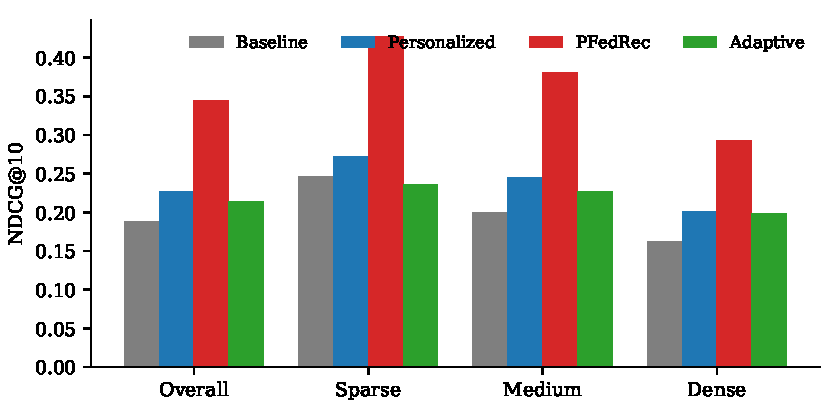
\includegraphics[width=0.9\linewidth]{figures/fig_group_bars.pdf}
  \caption{\ndcg{} of the four placements overall and by user group (best round, full
  population).}
  \label{fig:group-bars}
\end{figure}

First, keeping the user vector on the device is worth \GainPersonalizedVsBaselinePct\% \ndcg{}
over averaging it (\NdcgBaseline{} to \NdcgPersonalized) and
\GainPersonalizedVsBaselineSparsePct\% on sparse users, in the one pair of runs that differ in
nothing else (same loss, dimension, optimiser, learning rate, strategy and seed). Second, the
private head on a shared item table is far ahead of the three BPR-based placements
(\NdcgPfedrec{} against at most \NdcgPersonalized), and the ordering holds in every group. Third,
the adaptive blend is below the plain private user vector overall (\NdcgAdaptive{} against
\NdcgPersonalized) and, on the sparse group it was designed for, below even the all-global
baseline (\NdcgAdaptiveSparse{} against \NdcgBaselineSparse). The original hypothesis H1 is
refuted on this run.

\pending{paired per-user Wilcoxon tests with Holm correction and effect sizes for the six pairs
of methods, overall and by group; requires per-user scores of the Baseline, Personalized and
Adaptive runs (Section~\ref{sec:setup-stats}). Until then the differences in
Table~\ref{tab:main} are point estimates from one seed}.

\section{Best Round versus Last Round}
\label{sec:res-last-round}

Table~\ref{tab:last-round} places the in-loop metric at the selected best round and at round
\NRounds{} next to the full-population number. The ordering of the methods is the same at round
\NRounds{} as at the best round. The Personalized run peaks early (round
\RunPersonalizedBestRound) and its in-loop metric at round \NRounds{} is below its peak, while
the other three peak at round 83 and are close to their last-round value.

\begin{table}[htbp]
  \caption{Best-round and last-round \ndcg. In-loop columns are computed on the
  \ClientsPerRound{} clients sampled in that round; the full-population column at round \NRounds{}
  requires a re-score from the round-\NRounds{} checkpoint.}
  \label{tab:last-round}
  \centering\scriptsize
  % AUTO-GENERATED by thesis/scripts/build_assets.py -- do not edit by hand.
% eval_metrics_history (in-loop, sampled clients) vs final_metrics.best; full-pop round-100 column pending
\begin{tabular}{lrrrrr}
\toprule
Method & Best round & NDCG@10 best (6040 users) & In-loop NDCG@10 at best round (604) & In-loop NDCG@10 at round 100 (604) & Full-population NDCG@10 at round 100 \\
\midrule
Baseline (all-global BPR-MF) & 83 & 0.1882 & 0.2112 & 0.1556 & \pending{round-100 re-score} \\
Personalized (split learning) & 33 & 0.2275 & 0.2572 & 0.2482 & \pending{round-100 re-score} \\
PFedRec (+ final calibration) & 83 & 0.3447 & 0.3562 & 0.3436 & \pending{round-100 re-score} \\
Adaptive (dual-level, $\alpha$ blend) & 83 & 0.2144 & 0.2362 & 0.2342 & \pending{round-100 re-score} \\
\bottomrule
\end{tabular}

\end{table}

\begin{figure}[htbp]
  \centering
  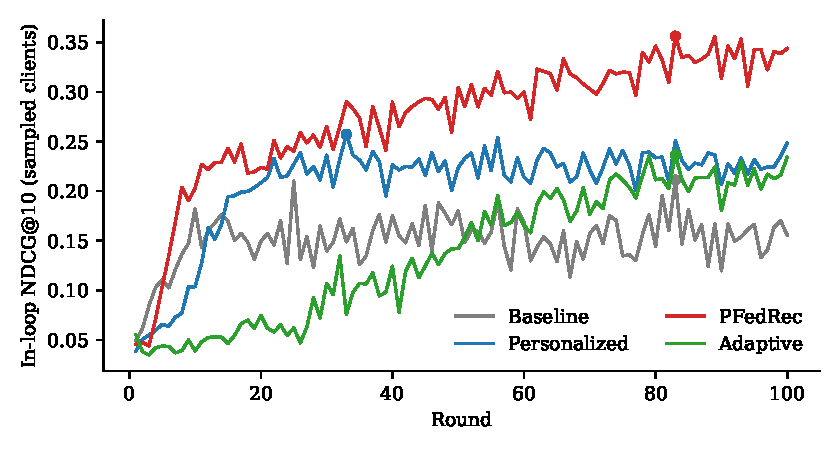
\includegraphics[width=0.9\linewidth]{figures/fig_training_curves.pdf}
  \caption{In-loop \ndcg{} of the sampled clients per round; the marker is the selected best
  round of each run.}
  \label{fig:training-curves}
\end{figure}

\section{Where Does the Value of Personalisation Live? Counterfactual Heads}
\label{sec:res-placement}

Table~\ref{tab:head-counterfactuals} and Figure~\ref{fig:head-counterfactuals} re-score the
PFedRec run with the item table, the bias and the 100 candidates per user held fixed and only
the head replaced (Section~\ref{sec:method-reeval}).

\begin{table}[htbp]
  \caption{Counterfactual heads on the PFedRec run \RunPfedrecShort. Every row scores the same
  item table and the same candidates; only the head differs. The blend row uses the
  hierarchical-conditional $\alpha_u$ rule of the adaptive method (mean $\alpha_u=\HeadAlphaMean$,
  range \HeadAlphaMin--\HeadAlphaMax).}
  \label{tab:head-counterfactuals}
  \centering\small
  % AUTO-GENERATED by thesis/scripts/build_assets.py -- do not edit by hand.
% reeval_<variant>_best.json of run cf72e0; same globals, same 100 candidates per user
\begin{tabular}{lrrrrrr}
\toprule
Head used at scoring time & NDCG@10 & $\Delta$ vs.\ own head & Sparse & Medium & Dense & HR@10 \\
\midrule
Own calibrated head $w_u$ (reference) & 0.3447 & -- & 0.4270 & 0.3802 & 0.2935 & 0.6111 \\
Blend $\alpha_u w_u + (1-\alpha_u)\bar w$, hierarchical-conditional $\alpha_u$ & 0.3061 & -0.0386 & 0.3483 & 0.3188 & 0.2842 & 0.5545 \\
Population-mean head $\bar w$ (uniform mean of 6040 heads) & 0.2510 & -0.0937 & 0.3113 & 0.2678 & 0.2208 & 0.4518 \\
Population head, weighted by interaction count & 0.2375 & -0.1072 & 0.2874 & 0.2550 & 0.2097 & 0.4373 \\
Another user's head (random permutation) & 0.1973 & -0.1474 & 0.2476 & 0.2126 & 0.1711 & 0.3727 \\
Freshly initialised head per user & 0.0741 & -0.2706 & 0.0725 & 0.0808 & 0.0692 & 0.1522 \\
One shared freshly initialised head & 0.0150 & -0.3297 & 0.0070 & 0.0135 & 0.0184 & 0.0291 \\
\bottomrule
\end{tabular}

\end{table}

\begin{figure}[htbp]
  \centering
  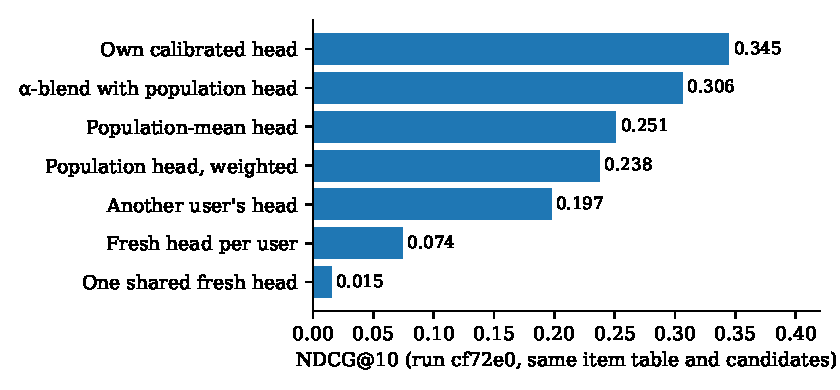
\includegraphics[width=0.85\linewidth]{figures/fig_head_counterfactuals.pdf}
  \caption{\ndcg{} of the counterfactual heads on the PFedRec run.}
  \label{fig:head-counterfactuals}
\end{figure}

The private head is load-bearing: the population-mean head costs \AbsDeltaHeadGlobalHead{}
\ndcg{} overall and the loss is largest in the sparse group (\NdcgPfedrecSparse{} to
\NdcgHeadGlobalHeadSparse), the group a population head is supposed to help. Another user's
head is worse still (\NdcgHeadShuffled), so the heads are personal and not merely a shared
offset. Blending does not help: the best single $\alpha$ on the grid is
$\alpha^\star=\HeadAlphaStarGlobal$ (the own head), and the data-driven rule of the adaptive
method, applied to this head, gives \NdcgHeadAlphaPolicyHc{} (\DeltaHeadAlphaPolicyHc), again
with the largest loss on sparse users (\NdcgHeadAlphaPolicyHcSparse). Hypothesis H3 holds on
this run. The two ``fresh head'' rows reproduce the cold-evaluation error of
Section~\ref{sec:setup-validity}: a freshly initialised head per user gives \NdcgHeadRandom{}
and one shared fresh head \NdcgHeadGlobalHeadCold, which is why a cold evaluation looks like a
broken model rather than like a crash. \pending{paired Wilcoxon tests of each row against the
own-head reference; the per-user scores of all rows are committed}.

\section{PFedRec: the Reproduction Gap and Post-tuning}
\label{sec:res-pfedrec}

The PFedRec paper reports \PublishedPfedrecNdcg{} \ndcg{} and \PublishedPfedrecHr{} \hr{} on
ML-1M; the reproduction under the thesis protocol gives \NdcgPfedrec{} and \HrPfedrec. The
official code run on the same machine and data gives \OfficialCodeNdcg{} and \OfficialCodeHr{}
(\pending{confirm the participation fraction, rounds and local epochs of that run}), so the gap
is not a machine or data artefact. Two protocol causes were put forward: the participation
fraction ($C=\ParticipationC$ here, $C=1$ in the paper) and the inference protocol (the official
code scores with a client-side post-tuned item table). The second cause was measured with the
registered experiment of Section~\ref{sec:method-posttune}.

\begin{table}[htbp]
  \caption{The three registered PFedRec rows (posttune README, rule fixed before the run) and
  the run without final calibration. Post-tuning rows use $E=1$, the official default; the
  $E=3$ cells are in Appendix~\ref{app:posttune}.}
  \label{tab:pfedrec-rows}
  \centering\small
  % AUTO-GENERATED by thesis/scripts/build_assets.py -- do not edit by hand.
% posttune/reeval_qu_diag_best.json baseline_metrics + metrics_by_cell (E=1 cells); ef41ab final_metrics.best
\begin{tabular}{lrrrrrr}
\toprule
Scoring protocol & NDCG@10 & Sparse & Medium & Dense & HR@10 & MRR \\
\midrule
PFedRec, scored with the shared item table (thesis number) & 0.3447 & 0.4270 & 0.3802 & 0.2935 & 0.6111 & 0.2821 \\
PFedRec, post-tuning, clean negatives ($E=1$) & 0.3181 & 0.4165 & 0.3611 & 0.2564 & 0.5584 & 0.2608 \\
PFedRec, post-tuning, official-code negatives ($E=1$) & 0.3789 & 0.4305 & 0.3891 & 0.3564 & 0.6642 & 0.3090 \\
\midrule
PFedRec without final calibration (run ef41ab, best round 100) & 0.3352 & 0.4057 & 0.3710 & 0.2870 & 0.5924 & -- \\
\bottomrule
\end{tabular}

\end{table}

Table~\ref{tab:pfedrec-rows} gives the registered three-row report. With clean negatives,
post-tuning \emph{lowers} \ndcg{} from \NdcgPfedrec{} to \NdcgEOneClean; with the official-code
negatives, which exclude the held-out test item, it \emph{raises} it to \NdcgEOneLeaky. The
paired statistics are in Table~\ref{tab:posttune-wilcoxon}, the per-group values in
Appendix~\ref{app:posttune}.

\begin{table}[htbp]
  \caption{Paired Wilcoxon tests of each post-tuning cell against the shared-table reference
  (\DsUsers{} users). $p$ one-sided tests the registered hypothesis ``cell $>$ reference'' with
  zero differences discarded; $p$ Pratt keeps them. Rows marked W$^-$=0 have no user whose score
  decreased, so their $p$-values follow from the construction (Section~\ref{sec:method-posttune})
  and the evidence is the confidence interval.}
  \label{tab:posttune-wilcoxon}
  \centering\scriptsize
  % AUTO-GENERATED by thesis/scripts/build_assets.py -- do not edit by hand.
% stats_wilcoxon.json cells.<cell>.by_scope.overall; n+/n-/n0 recomputed from the two per-user CSVs; W^-=0 marks p-values fixed by construction (< 1e-10); delta HR in the per-group table
\begin{tabular}{lrrrrrr}
\toprule
Cell & $\Delta$NDCG@10 [95\% CI] & $n_+/n_-/n_0$ & $p$ one-sided & $p$ two-sided & $p$ Pratt & $r$ \\
\midrule
$E=1$, clean & \mbox{-0.0266} \mbox{[-0.0315, -0.0217]} & 979/516/4545 & 1.0 & $9.5\times10^{-4}$ & $<10^{-10}$ & -0.099 \\
$E=1$, official-code & +0.0342 \mbox{[+0.0318, +0.0366]} & 1329/0/4711 & W$^-$=0 & W$^-$=0 & W$^-$=0 & +1.000 \\
$E=3$, clean & \mbox{-0.0685} \mbox{[-0.0757, -0.0613]} & 1281/1160/3599 & 1.0 & $<10^{-10}$ & 0.996 & -0.359 \\
$E=3$, official-code & +0.1073 \mbox{[+0.1026, +0.1122]} & 2502/0/3538 & W$^-$=0 & W$^-$=0 & W$^-$=0 & +1.000 \\
\bottomrule
\end{tabular}

\end{table}

\paragraph{Mechanism.} The candidates are items the user never interacted with, so their rows
in $\Qu$ change only when they are drawn as training negatives, and then they are pushed down.
With clean negatives the test item is drawn like any other candidate; when it is, the user's
test item falls out of the top 10 and that user's \ndcg{} becomes exactly $0$. At $E=1$ this
happened to \PtZeroLosersEOneClean{} users, all of whom have \ndcg{} $=0$ and a touched test
row, while \PtNPosEOneClean{} users gained a little because some of their 99 negatives were
pushed down. The mean therefore falls (\PtDeltaEOneClean, CI \PtCiEOneClean) while the rank
test under Pratt's rule, which weighs the many small gains, points the other way
(\PtPPrattEOneClean); the registered one-sided test (\PtPOneEOneClean) and the two-sided test
(\PtPTwoEOneClean) agree with the mean. Both are reported; the thesis uses the mean with the
mechanism stated. \decision{whether the thesis criterion for ``clean post-tuning hurts'' is the
mean with CI, or the rank test; recommendation: report both, conclude on the mean}.

With the official-code negatives the test item is never drawn, so no user can lose
($n_-=\PtNNegEOneLeaky$) and every touched candidate helps. Figure~\ref{fig:posttune-delta}
shows the two per-user distributions.

\begin{figure}[htbp]
  \centering
  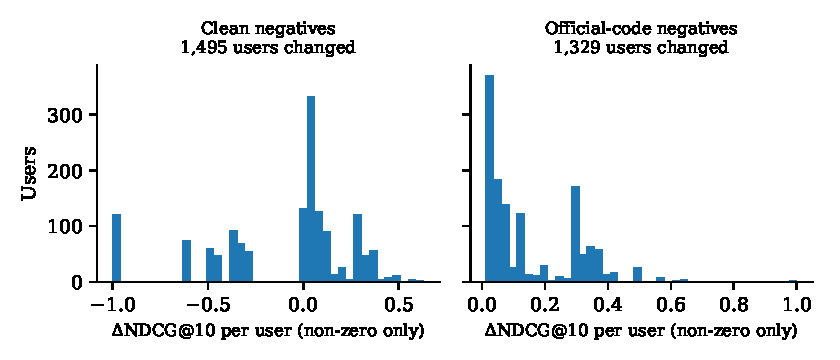
\includegraphics[width=0.9\linewidth]{figures/fig_posttune_delta.pdf}
  \caption{Per-user change of \ndcg{} after one post-tuning epoch, clean negatives (left) and
  official-code negatives (right); users with no change omitted.}
  \label{fig:posttune-delta}
\end{figure}

\paragraph{The size of the leak.} The two trajectories of a user differ only in the draws that
hit the test item, so the contrast official $-$ clean is non-zero for exactly
\PtContrastEOneNonZero{} users at $E=1$ and \PtContrastEThreeNonZero{} at $E=3$
(Table~\ref{tab:posttune-contrasts}). The overall difference of \PtContrastEOne{} \ndcg{}
(CI \PtContrastEOneCi) is therefore an average of about \PtContrastEOnePerUser{} \ndcg{} per
affected user: drawing the test item once as a negative is enough to remove it from the top 10.
The effect is concentrated in dense users (\PtContrastEOneDense{} against
\PtContrastEOneSparse{} for sparse users), who have more interactions and therefore more draws.

\begin{table}[htbp]
  \caption{Contrast between the official-code and the clean negative pool at the same number of
  post-tuning epochs; $n_{\neq 0}$ is the number of users whose two trajectories differ.}
  \label{tab:posttune-contrasts}
  \centering\small
  % AUTO-GENERATED by thesis/scripts/build_assets.py -- do not edit by hand.
% stats_wilcoxon.json contrasts.<A>__minus__<B>.by_scope; n_neq0 from the per-user CSV
\begin{tabular}{llrrrr}
\toprule
Contrast & Group & $\Delta$NDCG@10 (official $-$ clean) & 95\% CI & $p$ one-sided & $n_{\neq 0}$ \\
\midrule
$E=1$ & overall & +0.0608 & \mbox{[+0.0558, +0.0658]} & W$^-$=0 & 639 \\
$E=1$ & sparse & +0.0141 & \mbox{[+0.0078, +0.0213]} & $2.8\times10^{-5}$ & 21 \\
$E=1$ & medium & +0.0281 & \mbox{[+0.0225, +0.0338]} & W$^-$=0 & 108 \\
$E=1$ & dense & +0.1000 & \mbox{[+0.0913, +0.1090]} & W$^-$=0 & 510 \\
\midrule
$E=3$ & overall & +0.1758 & \mbox{[+0.1677, +0.1838]} & W$^-$=0 & 1,694 \\
$E=3$ & sparse & +0.0404 & \mbox{[+0.0295, +0.0524]} & $<10^{-10}$ & 55 \\
$E=3$ & medium & +0.0781 & \mbox{[+0.0692, +0.0875]} & W$^-$=0 & 295 \\
$E=3$ & dense & +0.2915 & \mbox{[+0.2780, +0.3046]} & W$^-$=0 & 1,344 \\
\bottomrule
\end{tabular}

\end{table}

\paragraph{Consequence for the limitation statement.} The registered rule selected the
sentence: \emph{part of the gap to the published number comes from the official code excluding
the test item from the training negatives during post-tuning}. Post-tuning itself, with clean
negatives, does not close the gap; it widens it. The row with the official-code negatives
(\NdcgEOneLeaky) is still \GapLeakyEOneToPublished{} below the published number, a residue
not separated between $C$ and the deviations K1--K3 of
Table~\ref{tab:posttune-deviations}. The $E=3$ cell with official-code negatives reaches
\NdcgEThreeLeaky, above the published \PublishedPfedrecNdcg{} already at $C=\ParticipationC$;
it refuted prediction A5 and is reported only as a diagnostic of the protocol, not as a result
of the method. \decision{cite the $E=3$ official-code cell in the appendix and limitations only
(recommended) or omit it}.

\section{The Adaptive Method as a Negative Result}
\label{sec:res-adaptive}

The adaptive method ranks third overall and last on sparse users (Table~\ref{tab:main}). Three
causes were identified; two are measured here and one in Section~\ref{sec:res-privacy}.

\paragraph{The blending weight pulls taste toward the mean.} The counterfactual of
Section~\ref{sec:res-placement} applies the same hierarchical-conditional rule to the PFedRec
head and loses \AbsDeltaHeadAlphaPolicyHc{} \ndcg{}, most on sparse users, where the rule assigns
the lowest $\alpha_u$ (mean $\alpha_u = \HeadAlphaMean$ overall). On the grid, the best single
weight is the fully local one. This is indirect evidence, measured on the PFedRec head rather
than on the adaptive run's user vector; \pending{direct measurement on the adaptive run: the
distance of the blended vector $\tilde{\vect{p}}_u$ to the prototype and to $\pu$ by group, and
a re-score with $\alpha_u=1$ (no blend) from the run's cached state}.

\paragraph{The per-user network is too large for the data.} The PersonalMLP has
\ParamsPersonalMlp{} private parameters per client, trained on a median of \DsMedianRatings{}
interactions and on at most \ExpectedParticipations{} participations in expectation, each of
one local epoch. \pending{parameters-per-interaction by group and, if time permits, a re-score
with the MLP branch zeroed from the cached state}.

\paragraph{Uploading the user vector weakens privacy.} Section~\ref{sec:res-privacy}.

\section{Privacy and Communication}
\label{sec:res-privacy}

Table~\ref{tab:params-comm} gives the parameters each placement aggregates, keeps private, and
uploads per participation, derived from the architectures. The private-head placement uploads
the least (\ParamsPfedrecGlobal{} parameters), the split-learning placements about twice as
much, and the all-global baseline \ParamsBaselineGlobal, including every user vector. The
adaptive method uploads the global part plus the \ParamsAdaptiveUploadExtra{} floats of $\pu$.

\begin{table}[htbp]
  \caption{Parameters per placement. $^{\dagger}$Counted from the architecture; the measured
  size of the Flower messages is pending.}
  \label{tab:params-comm}
  \centering\small
  % AUTO-GENERATED by thesis/scripts/build_assets.py -- do not edit by hand.
% derived from federated_config dims (users 6040, items 3706); measured byte counts are pending
\begin{tabular}{lrrr}
\toprule
Method & Global parameters (aggregated) & Local parameters per client & Uploaded per participating client per round$^{\dagger}$ \\
\midrule
Baseline (all-global BPR-MF) & 633,491 & 0 & 633,491 \\
Personalized (split learning) & 240,891 & 65 & 240,891 \\
PFedRec & 118,593 & 32 & 118,593 \\
Adaptive (dual-level) & 240,891 & 197,701 & 240,955 \\
\bottomrule
\end{tabular}

\end{table}

\pending{byte-level table measured from the actual Flower messages (upload and download per
client per round, per method)}.

\pending{preference-reconstruction attack on the adaptive run: for every user, top-10 of
$\pu^\top\Qtab^\top$ over all \DsItems{} items versus the user's interacted items; hits overall
and by group against the random and popularity baselines; one paragraph on secure aggregation
as the mitigation and on why it does not cover the $\pu$ upload}.

\section{The Cost of Stale Private Parts}
\label{sec:res-staleness}

At the best round of the PFedRec run the median client was \StaleMedian{} rounds stale and
\StaleOverTen\% of the clients more than ten rounds (Figure~\ref{fig:staleness}). The cited run
calibrates every head for one epoch against the restored item table before scoring; the
otherwise comparable run without calibration (\RunPfedrecNocalShort, best round
\RunPfedrecNocalBestRound) scores \NdcgPfedrecNocal, a difference of \DeltaPfedrecCalibration{}
that is confounded by the best round (\RunPfedrecBestRound{} against
\RunPfedrecNocalBestRound) and by the code version. \decision{how to measure the stale-head
cost: (i) per-user \ndcg{} of the calibrated run against rounds since last participation;
(ii) re-score the Personalized run before and after one calibration epoch, paired, which
measures the same phenomenon on the user vector; (iii) keep the confounded run pair with the
confounds stated. Recommendation: (i) and (ii), with (ii) as the main measurement if the run's
saved state is available}. \pending{the chosen measurement, pre-registered before it is run}.
